\documentclass[border=4pt]{standalone}
\usepackage{pgfplots}
\pgfplotsset{compat=newest}

\begin{document}
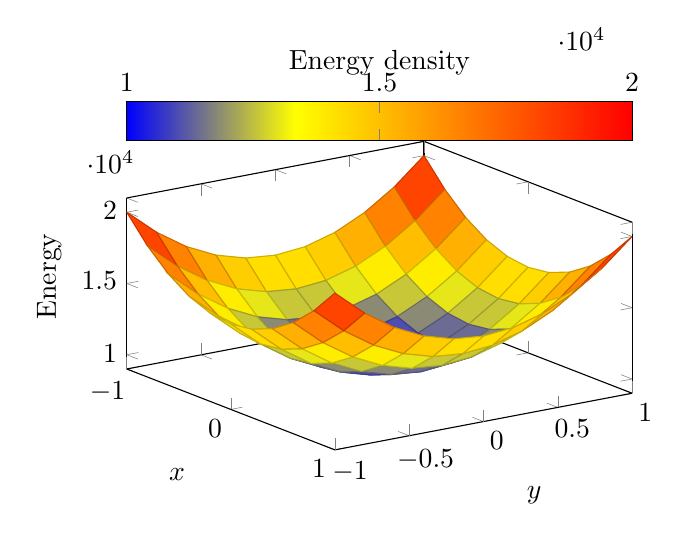
\begin{tikzpicture}
  \begin{axis}[
    width=8cm,
    height=5.5cm,
    view={55}{30},
    domain=-1:1,
    y domain=-1:1,
    samples=11,
    xlabel={$x$},
    ylabel={$y$},
    zlabel={Energy},
    colorbar horizontal,
    colorbar style={
      at={(parent axis.above north west)},
      anchor=south west,
      yshift=0.3cm,
      xtick={10000,15000,20000},
      xticklabel pos=right,
      title={Energy density}
    }
  ]
    \addplot3[surf] {10000 + 5000*(x*x+y*y)};
  \end{axis}
\end{tikzpicture}
\end{document}
